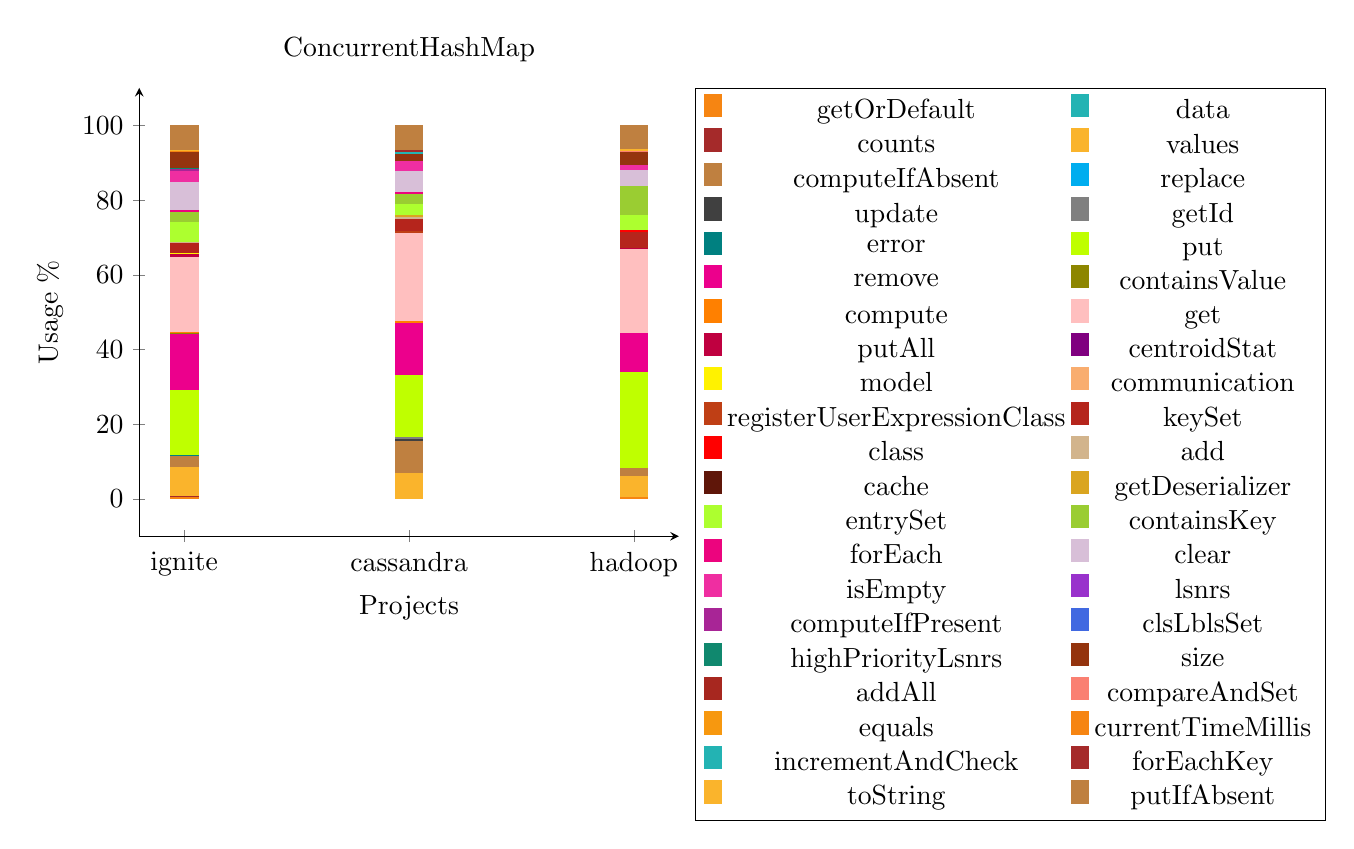
\begin{tikzpicture}
\begin{axis}[ybar stacked, axis x line=bottom, axis y line=left, enlarge x limits=true, enlarge y limits=true, grid=minor, xlabel={Projects}, ylabel={Usage \%},legend columns=2, legend pos=outer north east, xtick=data, xticklabels={ignite,cassandra,hadoop}, title={ConcurrentHashMap}]
\addplot[fill, color=BurntOrange] coordinates
    { (0,0.32) (1, 0.00) (2,0.43) };
\addplot[fill, color=TealBlue] coordinates
    { (0,0.11) (1, 0.00) (2, 0.00) };
\addplot[fill, color=Brown] coordinates
    { (0,0.11) (1, 0.00) (2, 0.00) };
\addplot[fill, color=Dandelion] coordinates
    { (0,7.86) (1,6.7) (2,5.63) };
\addplot[fill, color=brown] coordinates
    { (0,2.8) (1,8.76) (2,2.16) };
\addplot[fill, color=cyan] coordinates
    { (0,0.22) (1, 0.00) (2, 0.00) };
\addplot[fill, color=darkgray] coordinates
    { (0, 0.00) (1,0.52) (2, 0.00) };
\addplot[fill, color=gray] coordinates
    { (0, 0.00) (1,0.52) (2, 0.00) };
\addplot[fill, color=teal] coordinates
    { (0,0.11) (1, 0.00) (2, 0.00) };
\addplot[fill, color=lime] coordinates
    { (0,17.55) (1,16.49) (2,25.54) };
\addplot[fill, color=magenta] coordinates
    { (0,14.96) (1,13.92) (2,10.39) };
\addplot[fill, color=olive] coordinates
    { (0,0.11) (1, 0.00) (2, 0.00) };
\addplot[fill, color=orange] coordinates
    { (0,0.43) (1,0.52) (2, 0.00) };
\addplot[fill, color=pink] coordinates
    { (0,20.13) (1,23.71) (2,22.51) };
\addplot[fill, color=purple] coordinates
    { (0,0.65) (1, 0.00) (2,0.43) };
\addplot[fill, color=violet] coordinates
    { (0,0.11) (1, 0.00) (2, 0.00) };
\addplot[fill, color=yellow] coordinates
    { (0,0.11) (1, 0.00) (2, 0.00) };
\addplot[fill, color=Apricot] coordinates
    { (0,0.11) (1, 0.00) (2, 0.00) };
\addplot[fill, color=Bittersweet] coordinates
    { (0, 0.00) (1,0.52) (2, 0.00) };
\addplot[fill, color=BrickRed] coordinates
    { (0,2.58) (1,3.09) (2,4.33) };
\addplot[fill, color=Red] coordinates
    { (0, 0.00) (1, 0.00) (2,0.43) };
\addplot[fill, color=Tan] coordinates
    { (0,0.32) (1,0.52) (2, 0.00) };
\addplot[fill, color=Sepia] coordinates
    { (0,0.11) (1, 0.00) (2, 0.00) };
\addplot[fill, color=Goldenrod] coordinates
    { (0, 0.00) (1,0.52) (2, 0.00) };
\addplot[fill, color=GreenYellow] coordinates
    { (0,5.17) (1,3.09) (2,3.9) };
\addplot[fill, color=YellowGreen] coordinates
    { (0,2.91) (1,2.58) (2,7.79) };
\addplot[fill, color=RubineRed] coordinates
    { (0,0.32) (1,0.52) (2, 0.00) };
\addplot[fill, color=Thistle] coordinates
    { (0,7.53) (1,5.67) (2,4.33) };
\addplot[fill, color=Rhodamine] coordinates
    { (0,2.91) (1,2.58) (2,1.3) };
\addplot[fill, color=DarkOrchid] coordinates
    { (0,0.11) (1, 0.00) (2, 0.00) };
\addplot[fill, color=Mulberry] coordinates
    { (0,0.54) (1, 0.00) (2, 0.00) };
\addplot[fill, color=RoyalBlue] coordinates
    { (0,0.11) (1, 0.00) (2, 0.00) };
\addplot[fill, color=PineGreen] coordinates
    { (0,0.11) (1, 0.00) (2, 0.00) };
\addplot[fill, color=RawSienna] coordinates
    { (0,4.2) (1,2.06) (2,3.46) };
\addplot[fill, color=Mahogany] coordinates
    { (0,0.11) (1, 0.00) (2, 0.00) };
\addplot[fill, color=Salmon] coordinates
    { (0, 0.00) (1, 0.00) (2,0.43) };
\addplot[fill, color=YellowOrange] coordinates
    { (0,0.11) (1, 0.00) (2, 0.00) };
\addplot[fill, color=BurntOrange] coordinates
    { (0,0.22) (1, 0.00) (2, 0.00) };
\addplot[fill, color=TealBlue] coordinates
    { (0, 0.00) (1,0.52) (2, 0.00) };
\addplot[fill, color=Brown] coordinates
    { (0, 0.00) (1,0.52) (2, 0.00) };
\addplot[fill, color=Dandelion] coordinates
    { (0,0.11) (1, 0.00) (2,0.43) };
\addplot[fill, color=brown] coordinates
    { (0,6.89) (1,6.7) (2,6.49) };
\legend{getOrDefault, data, counts, values, computeIfAbsent, replace, update, getId, error, put, remove, containsValue, compute, get, putAll, centroidStat, model, communication, registerUserExpressionClass, keySet, class, add, cache, getDeserializer, entrySet, containsKey, forEach, clear, isEmpty, lsnrs, computeIfPresent, clsLblsSet, highPriorityLsnrs, size, addAll, compareAndSet, equals, currentTimeMillis, incrementAndCheck, forEachKey, toString, putIfAbsent};
\end{axis}
\end{tikzpicture}
